\chapter{Literature Review}
\label{chap:lit-review}
  \section{Space Exploration and NASA's Journey to Mars}
    \subsection{A Brief History}
      The human race possesses a trait that proposedly sets us apart from the majority of life forms around us; the powerful will to explore what is unknown. It is the curiosity and the thrill to push past the boundaries of what is thought to be possible, perhaps felt stronger by some, that forms the basis of many scientific endeavours relating to facts of life and existence around and outside of the immediate environment in which we live.
      
      A prime example of such a drive to explore is in the research and exploration of outer space, which, from a technological perspective, transitioned from astronomer's dream to scientist's and engineer's reality during the Cold War. Although space exploration as we know it today is motivated by human curiosity, it was during this period of political tension that significant breakthroughs in spacecraft and rocket propulsion technology were brought about. This period is referred to as the ``Space Race'' and stemmed from research and development of nuclear weaponry during World War II \cite[p. 147]{cornwell2003hitler}. The race began with the attempted launches of artificially made satellites \cite[pp. 3-5]{schefter1999the} and within the 40 years following the success of the USSR's \textit{Sputnik I} in 1957, the first object to be put into orbit by man, space technology progressed from early manned flights beginning in 1961\footnote{First human in space, Soviet launched} through the \textit{Apollo 11} lunar flight to having flown by of the majority of the planets in our solar system.
      
      By 1981, the launch of \textit{Columbia} \cite{williamharwood2009}, a space shuttle designed to be used for more than one flight, marked the beginning of reusable space technologies answering to the problem of cost and with the forethought of future increase in space flight frequency and demand. Today, the efforts to lower the cost of space travel and the attempt to bring space exploration into the private sectors to make these opportunities more realisable by the public are evident in Elon Musk's SpaceX development of the Falcon 9, a reusable rocket booster stage that returns and lands safely back on the surface of Earth \cite{spacex_popularmechanics}.
      
      The National Aeronautics and Space Administration (NASA) of the United States has been and still is responsible for a large chunk of mankind's search among the stars and, with respect to research and exploration, has made great efforts to better understand the planet that we live on in conjunction with the immediate spacial environment around Earth, the solar system and the planets within, and that which lies in deep space. After the Apollo lunar missions, efforts by NASA to explore involved one of the first space stations, the \textit{Skylab}, which suffered technical difficulties originating from launch but proved the ability to conduct research in space as well as allow astronauts to perform repairs and maintenance to artificial bodies in that environment \cite{compton1983living}. \textit{Skylab} was followed by the International Space Station (ISS), intended to be a more sustainable microgravity environment in which to conduct research that might require such conditions. Research of this type include a very broad range of investigations from the effects of near-weightlessness on plants and animals through to growth of human-like tissues and protein crystallisation \cite{nasaresearch}. An area of research that specifically relates to this project is in the development of technology to allow for longer, cheaper and faster flights in space, both in spacecraft materials and systems, and in astronaut health and performance. This is closely coupled with the search by entities around the world for other forms of life outside of Earth's atmosphere fuelled by the prospect of finding environmental architectures similar to ours. One of NASA's goals outlined in \cite{nasa2010act} is to send humans to Mars and this has lead to enormous amounts of research, promising engineering and technological successes that will ultimately allow humankind to extend civilisation across more than one planet.
    
    \subsection{Mars} 
      NASA has identified that Mars is a planet with greater similarity in formation and conditions in its history and as a result has been a target of exploration for more than 40 years. This has involved multiple flybys and orbits starting from 1962 through to the first lander, the \textit{Viking 1}, to touch down on the surface of the planet in 1975 \cite{marsprogram2008}. NASA's Jet Propulsion Laboratory (JPL) landed the spacecraft, named \textit{Pathfinder}, that contained the first successful rover vehicle, the \textit{Sojourner}, in 1997 \cite{pathfindersojournerjpl}. The purpose of this mission was to prove the possibility of cheaper spacecraft development and the transport of scientific equipment to the planet as well as taking photographs of the red surface, from the surface. 
    
      \texttt{***\\
      A short paragraph on current goals by NASA relating to modern Mars exploration and the need for rovers, to introduce the next section\\
      ***}
      
    % TODO: NASA and Mars
    % Something about why we need rovers and what was NASA's goal etc
    
  \section{The Mars Science Laboratory and Curiosity}
    \subsection{Overview}
      The Mars Science Laboratory (MSL) is a mission that was launched by NASA to further explore the surface of Mars, one of many orbiter, lander and rover type missions as part of the Jet Propulsion Laboratory's (JPL\footnote{Jet Propulsion Laboratory of California Institute of Technology}) Mars Exploration Program (MEP). The program is structured to work towards a set of goals to ultimately understand and determine the potential for life on Mars \cite{meptheme} by observation of the current climate and geology. The MSL is the latest mission in operation as part of MEP and was intended to span roughly one Martian year after touchdown on Mars. However, it has continued to operate for more than double that amount of time. 
      
      \begin{figure}[ht]
        \centering
        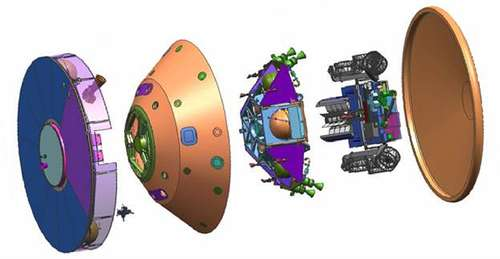
\includegraphics[width=0.7\textwidth]{figures/mslSpacecraftExplodedView.jpg}
        \label{fig:mslSpacecraftExplodedView}
        \caption[An exploded 3D model of the Mars Science Laboratory spacecraft including the cruise stage (far left) and heat shield (far right)]{An exploded 3D model of the Mars Science Laboratory spacecraft including the cruise stage (far left) and heat shield (far right) \cite{fig:mslSpacecraftExplodedView_cite}}
      \end{figure}
      
      
      MSL was launched from Cape Canaveral Space Station, Launch Complex 41, atop an Atlas V vehicle, a two stage rocket \cite{harwood2014sfn}. The mission required the launch vehicle to insert the five-piece MSL spacecraft into a transfer orbit in a process known as a Trans-Mars Injection (TMI) allowing the spacecraft to arrive at Mars after a 566 million kilometre trip that lasted 256 days. Figure~\ref{fig:mslSpacecraftExplodedView} shows a 3D render of the components of the spacecraft that made the trip. Four trajectory correction manoeuvres were made during the flight to result in a landing near ``Mount Sharp'' in Gale Crater, deemed the most accurate landing on Mars of any other spacecraft \cite{martinmur}.
      
      \texttt{***\\
      A piece on the choice of a landing site for Curiosity\\
      ***}
      % TODO: Launch site choice
    
    \subsection{Primary Mission Goals and Objectives}
      Touching down on the surface of Mars, the MSL had primary objectives tailored to contribute to the four goals as outlined in the MEP. The objectives were carried out by the MSL's flagship component, the Curiosity rover, and consisted of a wide range of biological and geological observations such as to determine the chemical building blocks that exist on the surface including organic carbon compounds, prospective historical biological activity, atmospheric processes of evolution, surface radiation and state and distribution of water \cite{mslobjectivesjpl}.
      
      Apart from the primary objectives, the MSL mission pushes further the boundaries of space exploration in that it proved the ability to land heavier vehicles at incredibly precise landing accuracy as well as the achievement of wider surface coverage to collect and observe more diverse samples of the surface of Mars.
              
    \subsection{Curiosity Technical Breakdown}
      23\% of the MSL spacecraft's total mass of 3.893 metric tonnes was thanks to the missions vehicle, \textit{Curiosity}. The six wheeled, instrument-bearing rover features much improved hardware over previous vehicles along with a multiple systems of new instruments to enable the carrying out of the mission objectives.
      
      The mechanical and technological specifications are broken down in the sections that follow.
      
      \subsubsection{Mechanical Structure}
        Structurally, \textit{Curiosity} comprises of mechanical features and principles borrowed from the previous three rovers, \textit{Sojourner}, \textit{Spirit} and \textit{Opportunity}, however, was made much larger (almost double the size). The reason behind the increase in size was the need for extra volume in which to fit the significantly larger set of scientific instruments, 100 times larger than the suite on \textit{Sojourner} \cite{planetary2011}.
        
        ![Body structure image]
        
        The body of the rover, a shallow, rectangular box, dominates its structural layout and serves as the central feature onto which all others subsystems are mounted. The chassis is also host to some of the rover's scientific instruments as well as the avionics box. The electronics that make up the avionics operate in a warm environment \cite{nasajulypresskit}, thus requiring the body to provide thermal insulation from the external conditions of Mars, giving it the name the Warm Electronics Box (WEB). The regulation of internal temperature, aided by the use of electrical heaters, is taken care of by a heat rejection system involving a pumped-fluid loop with the source of heat being the power generator, discussed in a section to follow. Thermal regulation also widened the range of potential landing sites with respect to their distance from the equator.
        
        Overall, \textit{Curiosity} was designed to exceed normal standards of mechanical robustness given the fact that hand-on maintenance is not a possibility when operating so far away from Earth. All subsystems on the rover minimised the opportunity for accidental collisions that might result in unfixable damage to the subsystems and thus jeopardy of the entire mission. In addition to the stringent design procedures, complex simulations of the rover's mechanical operation were done in virtual environments which allowed engineers to ensure, as far as possible, the success of the design in the differing environment that is on the surface of Mars.
        
      \subsubsection{Manoeuvrability}
      \label{subsubsec:lit-manoeuvrability}
        One of the main similarities between \textit{Curiosity} and its predecessors is the mechanical subsystem that provides the rover's ability to move around the surface of the planet. The six wheels, each half a meter in diameter, are constructed from aluminium with titanium spokes specially designed to allow for an amount of flexibility required for shock absorption and support. Protruding from the skin of the wheels are cleats in the shape of chevrons. This is an improvement over previous rovers where the cleats were horizontal, a flawed design in that sideways slippage was possible. The angled nature of the chevron cleats on the wheels of the \textit{Curiosity} aimed to prevent this motion. The thin, tubeless design allowed the wheels to be as light as possible which is important not only for driving on soft parts of the Martian landscape (termed ``floating''), but also for the unique landing sequence the rover had to carry out. The significant increase in the total weight of \textit{Curiosity} meant that conventional means of landing, such as the use of air-cushion support, was not possible. The MSL leveraged the mechanical suspension subsystem on its rover for touchdown instead of providing a separate lander itself. Here, the springy wheel design helped minimise the damage brought about by the impact. As far as weight minimisation of the wheels was concerned, during the moments before the rover was released to land on the surface, the wheels were deployed in a dynamically stressful fashion from their folded position kept during flight. The deployment was sudden and extra weight would have increased the already significant forces imparted on the suspension subsystem during this manoeuvre \cite{planetary2014}.
        
        However, the feature that is definitive of current and previous Mars mobility systems is the structural arrangement of the wheels in the mechanical suspension subsystem. Each wheel is mounted to an end of the mechanical linkage design based on the ``rocker-bogie'' principle. On each side of the rover, the linkage consists of two pivoting beams, one mounted to the side of the rover body, named the ``rocker'' and the other mounted to the middle-facing end of the rocker, called the ``bogie''. The front-facing end of the rocker and both ends of the bogie each host a wheel structure which consists of a pivot and strut for the front and rear wheels and a strut for the middle wheel. Both mount points allow for rotation of the beams such that, to a certain extent, the linkage as a unit remains level despite uneven terrain. This means that any of the three wheels on a side of the rover may lift due to an obstacle, up to the size of the wheel itself, without any of the other wheels lifting off the ground. This results in the obvious benefit of a maximisation of stability, minimisation of angular displacement of the rover body and maximisation of wheel contact with the surface of Mars. Figure~![] shows one of the sides of the mobility system.
        
        ![RockerBogie image]
        
        In addition to the freedom of movement of each wheel, the rocker beams from both sides of the rover are connected via a differential bar mounted atop the rover body. The bar, which pivots about a central point on the deck of the body, limits the relative movement of the rocker beams such that one rocker will rotate absolutely in the opposite direction of the other. This significantly reduces the amount of tilt and pitch the body experiences when wheels on one corner of the rover are lifted above the other corners as well as maintains even load across all wheels. In addition, the differential provides the second axis of stability needed to keep the body from toppling forward or backwards about the rocker pivot points.
        
        All six wheels have drive motors that may act independently with each motor mounted to a strut. The four corner wheels' struts are connected to a pivot, actuated by a highly geared motor to allow independent rotation for steering. The configuration allows for \textit{Curiosity} to turn conventional arcs as well as turn on the spot, an advantage for its mobility. Priority was not placed on speed for the drive motors but rather they were designed to provide high torque for robustness and for travelling on Martian terrain. The maximum speed of \textit{Curiosity} is approximately 4 centimetres a second \cite{msllegsandwheels}.
        
        The mechanical mobility systems are coupled with the advanced navigational system aboard the rover, a pairing between an arrangement of navigational cameras and software. Four pairs of black and white ``Engineering Hazard Avoidance Cameras'' (Hazcams) with a field of view of approximately 120 degrees are positioned at the lower front and rear of the rover body, providing the rover with awareness of obstacles. The pairs of cameras create 3-dimensional maps of the terrain in front of and behind the rover. Together with the aid of this environmental mapping, two additional pairs of cameras with a much narrower field of view, namely the ``Engineering Navigation Cameras'' (Navcams), are mounted to the mast of the rover to provide a complementary perspective of the terrain.
             
      \subsubsection{Rover Compute Element}
        At the heart of \textit{Curiosity} is the computational entity responsible for control of all systems on-board the rover as well as facilitation of communications with the team on Earth. This set of pairwise redundant computers is called the ``Rover Compute Element'' (RCE) which contains more memory than previous rovers and is hardened against the effects of radiation from the outside environment. The RCE makes use of a \textit{RAD750} CPU designed by IBM and manufactured by BAE Systems Electronics, the radiation-hardened version of the \textit{PowerPC 750}. The \textit{RAD750} has a clock frequency of 110-200 MHz providing more than 266 MIPS of processing power. The pair redundancy of the RCE is such that one of the ``sides'' of the RCE is operating at a time while the other side kept in ``cold backup''. A software feature named ``second chance'' was built into the system whereby the alternate side of the RCE could take over basic control during the critical moments of the MSL's entry, descent and landing should the primary side fail \cite{nasajulypresskit}. During the flight to Mars, multiple versions of the entry, descent and landing software was sent to the spacecraft as improvements to the complicated procedure. After the landing, the original software was replaced by one which included control of the rover specifically on and around the surface of Mars. The RCE did not have enough memory to accommodate both flavours of the governing software and as such, each was installed at different points during the mission \cite{cnn2012milesoff}.
        
        The RCE software involves the use of a real-time operating system (RTOS) approach to core scheduling and operation. JPL opted for a COTS solution for the RCE software and used an RTOS product from Wind River Systems called VxWorks. The operating system was first released in 1987 and has been used in multiple industries from space and defence to consumer electronic and automotive applications \cite{electronicsdesign2011vxworks}, not to mention having been a part of 20 previous JPL's missions. Over the years, VxWorks has been improved in areas of modularity and upgradeability and offers a wide variety of application layers aimed at the Internet of Things. The choice by JPL, yet again, to use VxWorks on the RCE was motivated by the operating system's reliability and maturity, an extensive set of supporting tools and low-level scheduling hooks for critical real-time operations \cite{extremetech2012insidecuriosity}.
        
      \subsubsection{Additional Internal Systems}
        Stemming from the central control principle of the RCE are other computing and sensory subsystems that monitor and maintain healthy operation of the rover. One of these systems is the Inertial Measurement Unit (IMU) which gives \textit{Curiosity} a rotational awareness about three axes: roll, pitch and yaw. It is used with the acquired 3D map of the rover's immediate surroundings to estimate the angular position of the rover during navigation and thus ensure that the rover is stable and safe.
        
        \textit{Curiosity} also has an internal control subsystem that monitors various measurements including temperature, power consumption, power storage and communication systems. The control loop will ensure that the rover remains operational and can produce warnings should any of the measurements be abnormal.
               
      \subsubsection{Communication}
        Communication with the rover from the ground station on Earth is arguably the most critical component of the mission besides the rover itself. It allows the upload of series of commands generated by the team together with the software here on Earth as well as the download of scientific data, rover telemetry and images to aid the team in keeping the rover geographically aware. The communication systems were designed to be redundant and to ensure good quality links despite challenges involving the Earth's and Mar's rotation about their own axes and obstructions as a result. Figure~\ref{fig:litreview-telecomsstructure} shows a depiction of the telecommunication system structure.
        
        \begin{figure}[h]
          \centering
          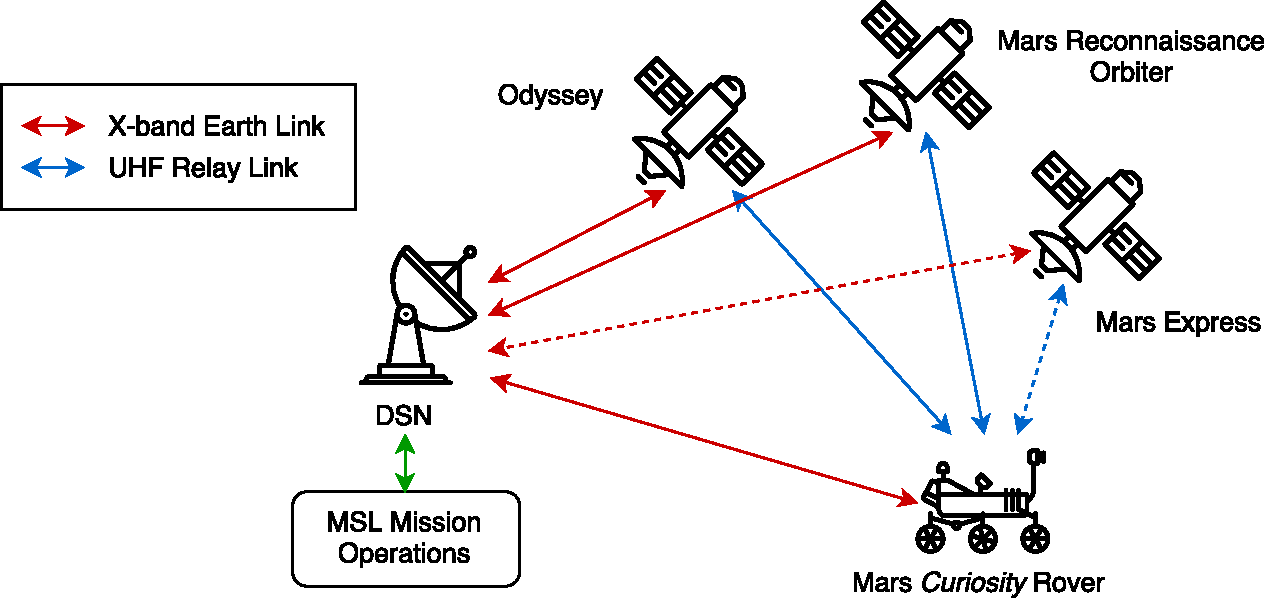
\includegraphics[width=0.71\linewidth]{figures/litreview-telecomsStructure}
          \caption[Diagram showing the structure of the MSL telecommunications system]{Diagram showing the structure of the MSL telecommunications system. Adapted from \cite{fig:litreview-telecomsstructure_cite}.}
          \label{fig:litreview-telecomsstructure}
        \end{figure}

        
        The Earth based component of this communication link originates from a collection of large antennas placed strategically around the Earth that alongside performing astronomical observation, provides communications for spacecraft that are travelling at an interplanetary scale. The system, a part of JPL, is called the NASA Deep Space Network (DSN) which consists of three facilities positioned in California, Spain and Australia \cite{jpldsnabout}. The positioning of the antennas in this way allows effective communication irrespective of the angular position of the Earth, meaning longer contact time between the team on Earth and \textit{Curiosity}. For JPL, the DSN is close to home and thus mainly hosts the central data hub for communications with the rover.
        
        On the Martian side of the link, the rover has aboard three antennas, two of which support the X-band\footnote{X-band - a radio frequency band within the microwave region (specifically between 8.0 and 12.0 GHz) used for engineering communication and radar} communication frequency and a third for Ultra-High Frequency (UHF) software radio communication. The X-band telecommunication system gives the rover a direct communication connection between Mars and the DSN on Earth and consists of a high-gain antenna (HGA) and the Rover low-gain antenna (RLGA) \cite{jpltelecom}. The HGA is movable with two degrees of freedom allowing \textit{Curiosity} to point it accurately back at Earth. This antenna facilitates direct to Earth (DTE) command transmission and direct from Earth (DFE) telemetry at between 160 bps and 800 bps depending on the DSN station size. The RLGA is used mainly for contingency DFE commands and is kept as more of a redundant communication feature. Downlink communication via the RLGA is also possible but again used in case of primary communication failure.
        
        The main method of communication with the rover when on the surface of Mars, however, is via the UHF system which uses the currently operational Mars orbiter spacecraft, the Mars Reconnaissance Orbiter (MRO) and Odyssey, as relays to the DSN. Relaying communication via multiple spacecraft which are orbiting the planet means that less power for signal amplification is required from the rover itself and the time of coverage from the perspective of the DSN stations is increased because objects orbiting the planet are obstructed by the planet body for shorter periods of time. MRO is the primary relay and Odyssey remains the redundant relay for when MRO is unavailable, provided the significantly lower data transfer speed allowed data transfer within DSN time and UHF energy constraints.
        
      \subsubsection{Instrumentation}
        Scientific observation and investigation of the surface of Mars by the \textit{Curiosity} rover forms the crux of the MSL mission and the instruments aboard the rover are the tools with which JPL and NASA are doing such. The ten instruments, primarily scientific, hosted by the rover body, are each designed to perform specific tasks on different aspects of the rover's surroundings and samples from which it may acquire. The typical flow of investigation would be initiated by inspection of high resolution images from the rover's array of cameras. Features of interest are then located, navigated to and further inspected by the instruments mounted on the rover's robot arm and hand. Features may be inspected using those tools, or brought into the rover's body for further analysis, should that be required. Additionally, atmospheric features may be observed using the instruments design for these types of investigations.
        
        The range of instruments, as highlighted by the flow of investigation above, are split into four categories based on their method of contact with their subject. The list below shows the classification as mentioned and provides a short summary of each of the instruments.
        
        \begin{itemize}
          \item \textbf{Remote Sensing Instruments}
          \begin{itemize}
            \item \textit{Mastcam (Mast Camera)}: a suite of two fixed-focal length (FFL) cameras, one the Narrow Angle Camera (NAC) with a $5.1^{\circ}$ FOV and 100 mm focal length, and the other the Medium Angle Camera (MAC) with a $15^{\circ}$ FOV and a 34 mm focal length \cite{mslsciencecornermastcam}. Each camera contains 8 Gb of buffer memory able to store over 5 500 raw frames, as well have the ability to pass the images through a collection of filters. Both cameras, although different in their FOV, focal length and color filter specifications, were designed to work together to provide stereoscopic views of landscapes, rocks and structures and the atmosphere.
            \item \textit{ChemCam (Chemistry and Camera)}: a suite of two remote sensing devices, the Laser-Induced Breakdown Spectrometer (LIBS) and the Remote Micro-Imager (RMI) \cite{mslsciencecornerchemcam}. The LIBS is the first ever laser sensing device in the field of planetary science and has the ability to investigate the elemental breakdown of rocks and other material under its sub-millimetre beam, an advantage over other breakdown spectrometers in that it can target very specific points on the surface. The RMI, which images through the same telescope as the LIBS, provides context and a highly targeted visual on the point at which the LIBS is operating. The RMI has a very small FOV of 19 milliradians and can distinguish the LIBS target point at any range within that of the LIBS laser beam. ChemCam provides further advantage over other contact-based analysis devices in that the team can use it to take samples more often without the need of the already tricky terrain traversal of the rover.
          \end{itemize}
          \item \textbf{Contact Science Instruments}
          \begin{itemize}
            \item \textit{APXS (Alpha Partical X-ray Spectrometer)}: a compound instrument consisting of an electronics system situated in the body of the rover and a sensor module on the hand of the rover's robot arm. Spectral measurements are made by placing the sensor in direct contact with the material of interest, or up to 2 cm away from it, and observing X-ray emissions for a time between 15 min and 3 hours \cite{mslsciencecornerapxs}. The sensor will then transmit the resultant data to the rover which contains up to 13 spectra and additional engineering information. The APXS on this rover is a significant improvement over that on \textit{MER} with between three and six times the sensitivity for low and high atomic number elements respectively.
            \item \textit{MAHLI (Mars Hand Lens Imager)}: a focusable, high-resolution, colour camera positioned on the end of the robotic arm used to take close-up images of subjects on the surface in places to which the rest of the rover's cameras do not have access. The camera has a range of features which give it flexibility in the nature of subjects that it might capture, including night illumination, auto focus, focus stacking and video \cite{mslsciencecornermahli}. Other use cases include searching for UV material, sky imaging, sample observation, stereo-pair imaging and rover self-portraits (fault diagnosis and for education and outreach).
          \end{itemize}
          \item \textbf{Analytical Laboratory Instruments}
          \begin{itemize}
            \item \textit{CheMin (Chemistry and Mineralogy)}: an in-body chemical and mineral analyses instrument which operates using the principles of powder X-ray Diffraction (XRD) as well as X-ray Fluorescence (XRF) on a nominal (but not maximum) amount of 74 samples as delivered by the Sample Acquisition, Sample Processing and Handling system SA/SPaH \cite{mslsciencecornerchemin}. Drill or scoop samples from this system reach the CheMin's funnel system on the deck of the rover, piezoelectrically vibrated to ensure transfer of the sample. Sample material is filtered numerous times, initially in the CHIMRA sorting chamber and then through filters in the sample cell. Sample analysis can there-onwards take up to 10 hours. The primary goal of the analytical observations performed by the CheMin is to identify and assess the historic or even current presence of water in the samples in an attempt to better understand the state of Mars with respect to the possibility of life on the surface. Raw CCD frames of the diffraction patterns and histograms are processed on the rover and then sent via downlink transmissions with the possibility of indication of indicators of previous inhabitance by life forms.
            \item \textit{SAM (Sample Analysis at Mars)}: a collection of three instruments: the Quadrupole Mass Spectrometer (QMS), a Gas Chromatograph (GC) and a Tunable Laser Spectrometer (TLS) \cite{mslsciencecornersam}. The instruments can work together and separately for much the same reason as the CheMin in terms of the search for evidence of life forms, but with focus in the area of organic chemistry in general as opposed to just water. The analyses form part of five science and measurement goals outlined for SAM are tightly coupled to the core MSL mission goals, and involve a multitude of investigations into the state and history of formation and destruction of compounds to reveal indicators of previous life. The sample manipulation system (SMS) and Chemical Separation and Processing Laboratory (CSPL) provide a means for the samples to be in the correct state and to reach the three instruments. The two support devices ensure correct environments are maintained within SAM for the analysis of the samples.
          \end{itemize}
          \item \textbf{Environmental Instruments}
          \begin{itemize}
            \item \textit{RAD (Radiation Assessment Detector)}: a charged particle telescope, mounted to the deck of the rover, which analyses particles with the aim of obtaining and characterising the spectrum of particle radiation on Mars. This is done to estimate the amount of radiation a human would encounter if they were to be on the surface on Mars and further understand what this radiation may have meant for life on Mars above and below the surface \cite{mslsciencecornerrad}.
            \item \textit{DAN (Dynamic Albedo of Neutrons)}: an active/passive neutron spectrometer provided by the Russian Federal Space Agency with the aim of estimating hydrogen content in the subsurface layers when the rover is traversing the planet. Most of the measurements take place during short stops that the rover may make during these journeys, the longer the measurement time resulting in more accurate measurements \cite{mslsciencecornerdan}.
            \item \textit{REMS (Rover Environmental Monitoring Station)}: a pair of horizontally outward facing booms attached to the Remote Sensing Mast, below the Chemcam, as well as an additional sensor on the deck of the rover. The Instrument Control Unit (ICU) for the REMS is positioned inside the rover body. The booms, sitting approximately 1.5 m above the surface of Mars, record wind speed and direction, pressure, relative humidity, air temperature and ground temperature while the deck-bound Ultraviolet Sensor (UVS) ultraviolet radiation. The position of the booms relative to each other and to the rover and its RMS was carefully engineered such that the wind perturbation would be as minimal as possible, an attempt to keep the wind measurements as accurate as possible. The measurements that the REMS takes are systematic and 5 minutes of observation takes place every hour of every sol\footnote{sol - the duration of a solar day on Mars} regardless of what operational state the rover is in, with the sensors operating at a data frequency of 1 Hz. Energy constraints allow total use of the REMS for three hours a day, which means that the REMS may autonomously increase the length of any of the 5 minute measurement operations if an atmospheric event has been detected.
            \item \textit{MARDI (Mars Descent Imager)}: a FFL colour camera fixed to the body of the rover, pointing directly downwards, which is capable of taking 1600 x 1200 images used during the landing of the MSL spacecraft. The camera consists of a 90 degree circular FOV lens behind which sits a rectangular FOV sensor. The camera started taking images on command at the time of heat shield separation and continued to do so at 5 images per second until approximately 2 minutes after touchdown. Each image stored realtime into flash memory (for later transmission) can be compressed, also in realtime. The burst of images was used to provide geographical indication of the exact landing point of the rover and a framework within which engineers could base early operations. Downlink transfer of these images would have been in the form of thumbnails first and then a subset of full resolution images afterwards.
          \end{itemize}
        \end{itemize}
      
      \subsubsection{Power}
        Unlike conventional spacecraft and planetary space vehicles, \textit{Curiosity} is not powered using solar means but rather energy is in the form of heat given off by the decay of a radioactive isotope, plutonium-238 dioxide. 4.8 kg of the decaying material is hosted inside of the generator named a Multi-Mission Radioisotope Thermoelectric Generator (MMRTG) produced by Rocketdyne and Teledyne Energy Systems, assembled and tested by Idaho National Laboratory \cite{inlgovfuelingcuriosity}. The heat produced by this decay process is then converted into electrical energy through the use of thermocouple devices and excess heat is transferred to the rest of the rover body for heating, as mentioned in a previous section. The thermocouple has the advantage of being able to leverage the cold outer-space environment for the ``cold junction'', making RTGs well suited to interplanetary travel. Radioisotope Thermoelectric Generators (RTG) are not new to the space industry and provide missions the longevity and more consistent and reliable sources of power that one might require.
        
        ![Image of rear end of the rover, the position of the MMRTG]
        
        The design concept behind the MMRTG is a generator that is more flexible in its field of applications as well as one which includes a high degree of safety, a desirable design feature in any space technology. Another goal of the MMRTG design is to optimise the power level over a lifetime of 14 years whilst minimising its weight \cite{srpsmmrtg}.
      
    \subsection{Robot Sequencing and Visualisation Software}
      While many portions of the \textit{Curiosity's} operation and movement are autonomous and require little direct input from the control team on Earth, the ground station has ultimate control over the functioning of the rover, the set of tasks it carries out and the timing with which to do so. The team also requires the ability to assess the state of the rover, its geographical position and its configuration along with, at the very least, depictions of its immediate surroundings. JPL engineers and scientist achieve such control and awareness with a specially created software suite which has been progressively developed and further improved alongside and for multiple recent Mars rover missions. The Rover Control Workstation (RCW) was developed initially to control the earlier Mars rover vehicle, \textit{Sojourner} \cite{cooper1998driving}, and was later used as a basis upon which the \textit{MER} control suite was written, the Rover Sequencing and Visualisation Program (RSVP).
      
      The principle behind the RSVP involved the goal to maximise the use of each sol on Mars whilst relieving the requirement for operators on Earth to have to endure the asynchronous timing of sols and Earth days which was viewed as an operational constraint. Another issue was the fact that traversal of a rover on Mars resulted in the lack of knowledge of the vehicle's final position, requiring the downlink transfer of telemetry and analysis of that data upon which to plan further activities. This process introduced time lag and a suboptimal use of time for rover operation. The RSVP, along with the RCW, introduced a set of tools which make the daily command cycle a more optimal procedure, starting with the ability to rapidly interpret data received from the instruments on the rover and reconstruct the state of the rover in the most accurate way possible, presenting this depiction of state to the operator. This includes spatial positioning of the rover and the environmental context within which it is situated. Further, the RSVP provides rapid composition and simulation of commands to send to the rover, which will autonomously carry out the commands therefore freeing the operator from the time-frame of another planet.
      
      Thus, RSVP was designed around the concept of the downlink-uplink cycle and contained two parts, Data Analysis and Sequence Generation. The Data Analysis facilitated functions of state awareness and immersion broken down into the following features:
      \begin{itemize}
        \item \textbf{State Analysis}: Analysis of the data obtained by sensors on the rover body pertaining to the state of subsystems of the rover to result in an understanding of the overall state of the rover.
        \item \textbf{Image Browsing}: Review and processing of images taken by the rover's cameras allowing the user to construct mosaics of panoramic sequences.
        \item \textbf{Terrain Modelling}: Construction of a 3D model of the immediate terrain as acquired from the rover's stereoscopic imaging systems which can later be used to plan traversals and ensure safe paths on the surface of Mars.
        \item \textbf{Terrain Visualistion, Immersion and Telepresence}: The use of the constructed 3D model of the terrain to immerse the operator into the environment giving the operator a better understanding of the surface and the positional state of the rover.
      \end{itemize}
      
      The RSVP's second part involves the notion of intelligent Sequence Generation and a convenient and efficient process flow in the construction of sequences of commands to send to the rover \cite{1_wright_hartman_cooper_maxwell_yen_morrison_2006}. The range of commands that an operator can send to the rover is wide and these commands have varying target levels of operation and an associated variation in the level of autonomy as a result. An example of a very low-level, non-autonomous command might be to turn on a heater while a heavily autonomous, complex command might involve setting a target traversal destination and allowing the rover to construct a route based on sensor data and algorithms. Sequence generation follows a fairly comprehensive process initiated by a meeting of the group of operators whereby they will discuss the state of the rover and the aim of the particular day's events. Scenarios are analysed and weighed against the constraints of the situation. Further meetings are held to plan the detail of the activities agreed upon and to receive approval of the plans. The RSVP aids this process by allowing the team to input a draft of the set of sequences and outputting a simulation of the execution of such sequences. Distribution of the set of commands to all the teams involved allows understanding of the objectives and events by all parties and after the final sequence has been approved and the RSVP has completed validation of the sequence, the commands are built to be sent via uplink.
      
      The variant of the RSVP used for \textit{Curiosity} was confusingly renamed to the \textit{Robot} Sequencing and Visualisation Program and contains much the same principle of operation and software features as the RSVP used for MER. The RSVP, in both MER and MSL cases, is clearly separated into two program user-interface components. The sequence generation is carried out in the Robot Sequence Editor (RoSE) \cite{soseroverdrivingtools} which is aware of the wide set of commands and how they will affect the rover as well as the compilation of commands for uplink. A view of the RoSE is shown in Figure~\ref{fig:litreview-rose}. Visualisation is taken care of by the program component called HyperDrive host to a high-fidelity set of 3D and stereo Martian surface displays \cite{nasatechbrief2013rsvp}, and example of which is shown in Figure~\ref{fig:litreview-hyperdrivecrop}.
      
      \begin{figure}[H]
        \centering
        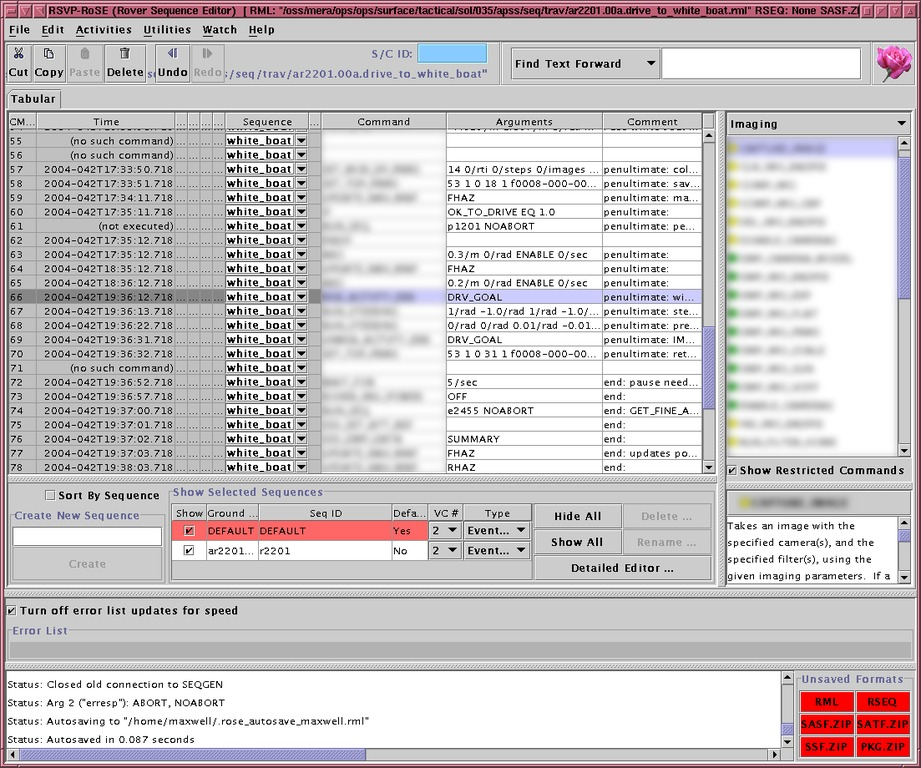
\includegraphics[width=0.7\linewidth]{figures/litreview-RoSE}
        \caption[A screenshot of the RoSE as implemented in the RSVP used for MER]{A screenshot of the RoSE as implemented in the RSVP used for MER \cite{fig:litreview-rose_cite}}
        \label{fig:litreview-rose}
      \end{figure}
      
      
      \begin{figure}[H]
        \centering
        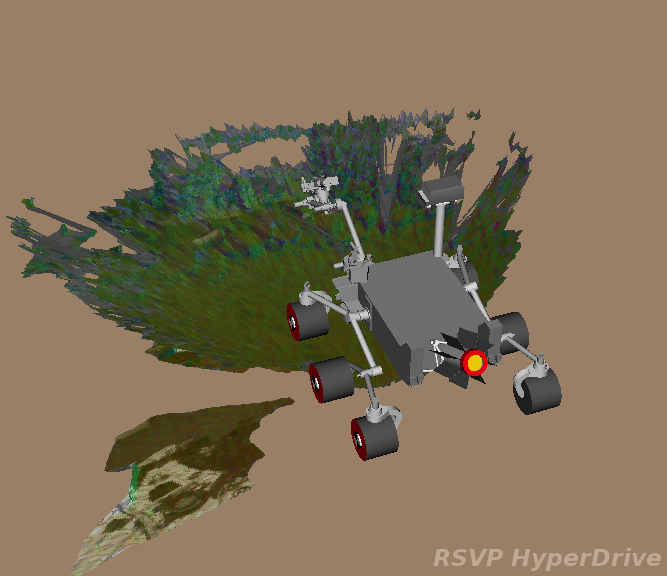
\includegraphics[width=0.7\linewidth]{figures/litreview-hyperdriveCrop}
        \caption[A view of the 3D model output by the RSVP HyperDrive program component for visualisation and immersion]{A view of the 3D model output by the RSVP HyperDrive program component for visualisation and immersion \cite{fig:litreview-litreview-hyperdrivecrop_cite}}
        \label{fig:litreview-hyperdrivecrop}
      \end{figure}


  \section{Space Education and Outreach}
  
  \section{Web Technologies for Modern Outreach}
    Until recently, the world of computers and their interconnectedness has been primarily a means of personal communication and collaborative, distributed computation with minimal focus on openly sharing information and educating. It has been with the exponential increase in performance and availability of communication and network technologies that the notion of mass sharing and consumption of information in a real-time sense has made a prominent standing in the way that the world makes use of the computational devices that they might possess.
    
    In recent years, online education has gained significant popularity due to the flexibility that it provides to the learner and the convenience to the educator. In 2001, MIT launched the OpenCourseWare initiative \cite{mit2001opencourseware} where learners may view educational content from MIT at no additional cost other than the cost of an internet connection by any means. UC Berkeley followed suit in 2006 along with Yale, Stanford and Harvard in later years and online education, beginning simply as a prospective endeavour, turned rapidly into the educationally rich internet that exists today. Multiple other organisations joined the fast growing culture, such as Kahn Academy, offering free education to those who have access to the internet.
    
    It is this ease-of-access that has driven the appeal of the web as a distributive platform for educational material. Institutions and organisations realised that education need not be hindered by the logistical constraints imposed on educators and that the web allowed them to educate learners in developing countries and other remote locations right from where they might be situated. They also realised that the material could be shared to a significantly larger audience compared to that in a classroom or lecture theatre. Today, advancements in web technologies and the progressive nature of current web standards means that the level of interactivity possible through a browser is only increasing.
    
    The web has, more recently, developed itself around a core culture of open source. It is the concept where development of a product or project can be accessed, used and contributed to, at no additional cost \cite{2_monago_2014}. Open source culture operates with a notion of constructive debate in collaboration in order to promote development and quality of the project and it inherently provides a highly educational environment in which people can tackle steep learning challenges with a positive and constructive outcome. Additionally, the availability of use of open source projects and culture make it possible for anyone to create and share a service or product on the internet with very little initial resources or funding required and it is this opportunity that many of the sources of online education have taken to their advantage. In a short amount of time, one can share large and complex forms of data securely and remotely for the benefit of others around the world.
  
  \section{Existing Curiosity Rover Models}